\documentclass[10pt]{report}

\usepackage{geometry}
\geometry{
	letterpaper,
	hmargin=1in,
	vmargin=1in,
	footskip=0.25in
}

\usepackage{enumerate} % for enumerate counter
\usepackage{subcaption} % for subfigures
\usepackage{amsthm} % for QED
\usepackage{mathtools} % for delimiter

\usepackage{listings} % for code
\lstset{ 
	language=R,
	basicstyle=\footnotesize\ttfamily,
	numbers=none,
	stepnumber=1,
	numbersep=8pt,
	showspaces=false,
	showstringspaces=false,
	showtabs=false,
	frame=single,
	tabsize=2,
	captionpos=t,
	breaklines=true,
	breakatwhitespace=false
} 

\usepackage{float} % for figure [H]
\usepackage{booktabs} % for tabular
\usepackage{caption} % for \caption*
\usepackage[export]{adjustbox} % for valign=t
\usepackage{array} % for column type m
\usepackage{verbatim}
\usepackage{graphicx}
%\graphicspath{ {imgs/} }

\usepackage{fancyhdr}
\pagestyle{fancy}
\fancyhead[L]{\hwAuther}
\fancyhead[C]{\courseNo}
\fancyhead[R]{\hwNo}

\usepackage{amssymb}
\usepackage{amsmath}

%Cover
\newcommand{\courseTitle}{Introduction to Mathematical Modeling}
\newcommand{\courseNo}{Math 380}
\newcommand{\hwAuther}{Zhihao Ai}

\newcommand{\hwNo}{HW \#6}
\newcommand{\hwDate}{Due on 03/13}

\title{
	\courseTitle\\
	\hwNo\\
	\hwDate
}
\author{\hwAuther}
\date{}
%

%Custom
%\everymath{\displaystyle}
\setlength\parindent{0pt}

%Custom commands
\newcommand{\ds}{\displaystyle}
\newcommand{\ts}{\textstyle}

\newcolumntype{N}{>$ c <$} 
\newcolumntype{M}[1]{>{\centering\arraybackslash $}m{#1}<{$}}

\newcommand{\abs}[1] {\left| #1 \right|}

\DeclarePairedDelimiter\autoparen{(}{)}
\newcommand{\pa}[1]{\autoparen*{#1}}

\newcommand{\var} {\text{var}}

\newcommand{\m}[1] {\mathbf{#1}}

\begin{document}

\maketitle

\begin{enumerate}
	\item [1a.]
	Let $b_i \in \{0,1\}, i=1,2,\dots,m$, s.t.
	\[
	b_i = 
	\begin{cases}
		0, & a_i \text{ is not chosen}\\
		1, & a_i \text{ is chosen}
	\end{cases}
	\]
	To restrict $x$ to take values only in the set, the linear constraints are
	\begin{align*}
		\sum_{i=1}^{m} b_i &= 1\\
		\sum_{i=1}^{m} a_i b_i &= x
	\end{align*}
	
	\item [2.]
	Below is the graph of the mainland states of Australia (Western Australia(WA), Northern Territory(NT), Queensland(Q), South Australia(SA), New South Wales(NSW) and Victoria(VC)):
	\begin{figure}[H]
		\centering
		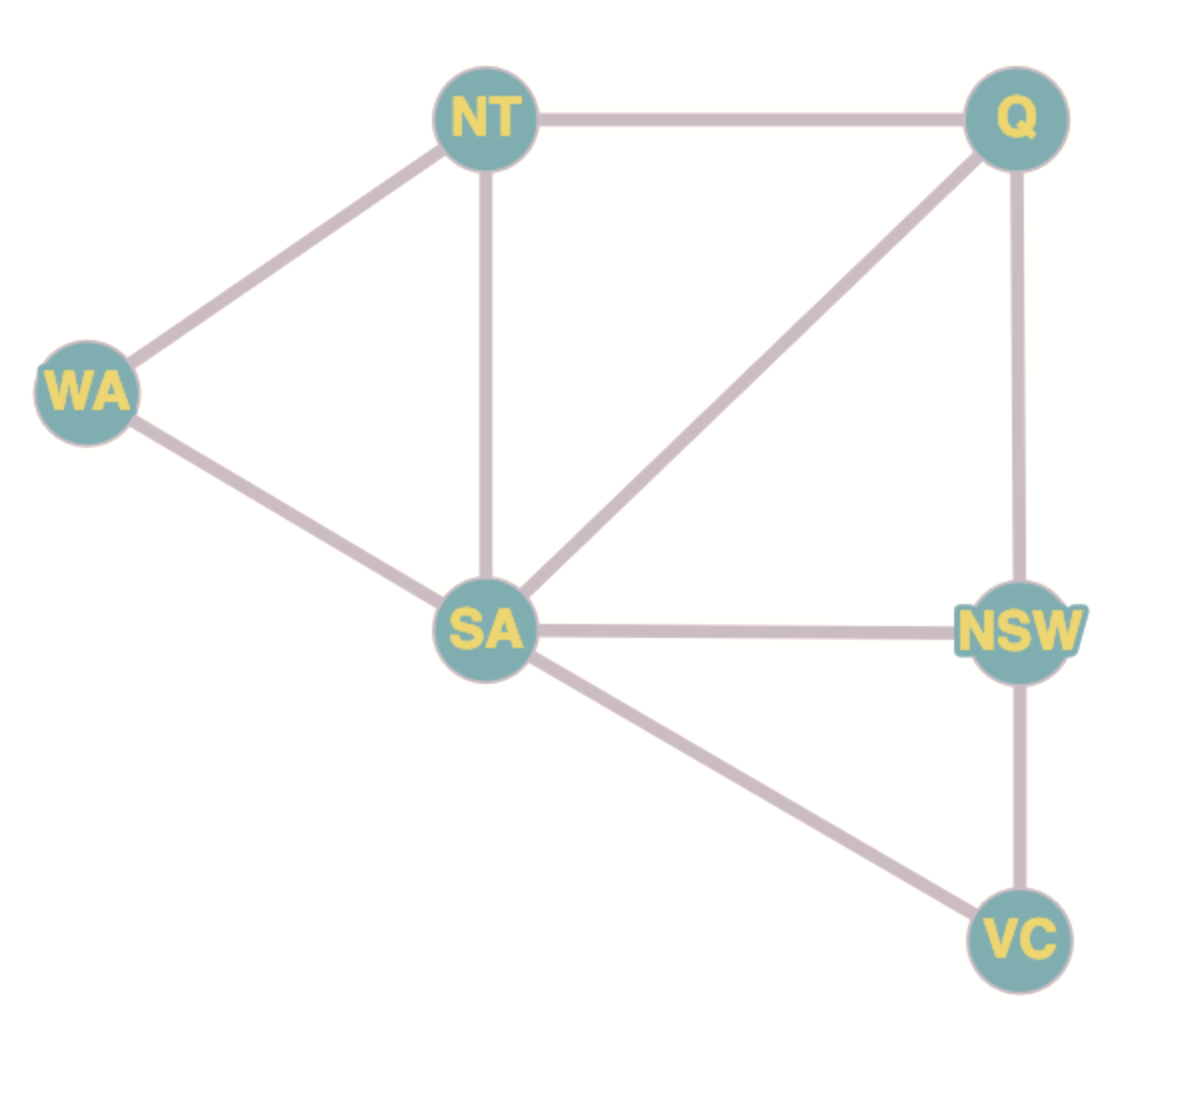
\includegraphics[width=0.35\linewidth]{2-1.png}
	\end{figure}
	It can be modeled mathematically as an undirected graph $G=(V, E)$ where
	\begin{align*}
		V &= \{VC, SA, WA, NT, Q, NSW\}\\
		E &= \{(WA, NT), (WA, SA), (NT, Q), (NT, SA), (Q, SA), (Q, NSW), (SA, NSW), \\
		&\qquad (SA, VC), (VC, NSW)\}
	\end{align*}
	The resulting graph is not Eulerian because there are vertices with odd degree.\\
	If Tasmania is added, the graph would become as follows:
	\begin{figure}[H]
		\centering
		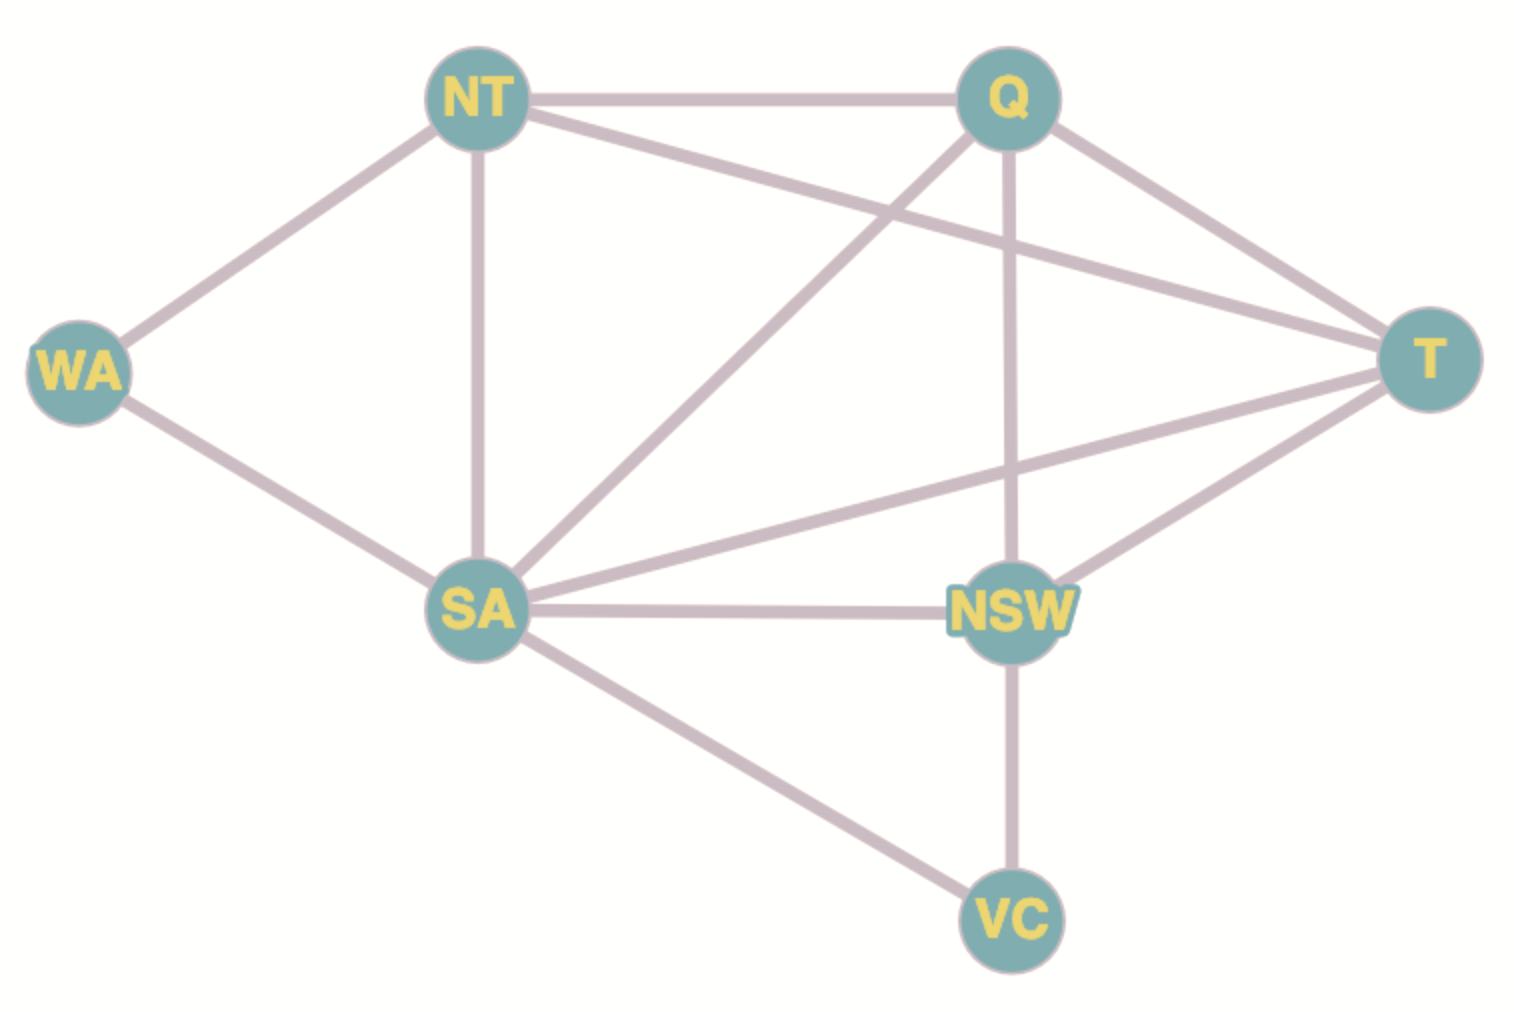
\includegraphics[width=0.4\linewidth]{2-2.png}
	\end{figure}
	The new graph is Eulerian. A walkabout can be $WA \to NT \to Q \to T \to NT \to SA \to Q \to NSW \to VC \to SA \to T \to NSW \to SA \to WA$.
	
	\item [3a.]
	\begin{enumerate}
		\item 
		Let the three colors be red($R$), green($G$) and blue($B$), then $v_i \in \{R,G,B\}, i=1,\dots,6$. Applying greedy algorithm on the graph, we have
		\begin{figure}[H]
			\centering
			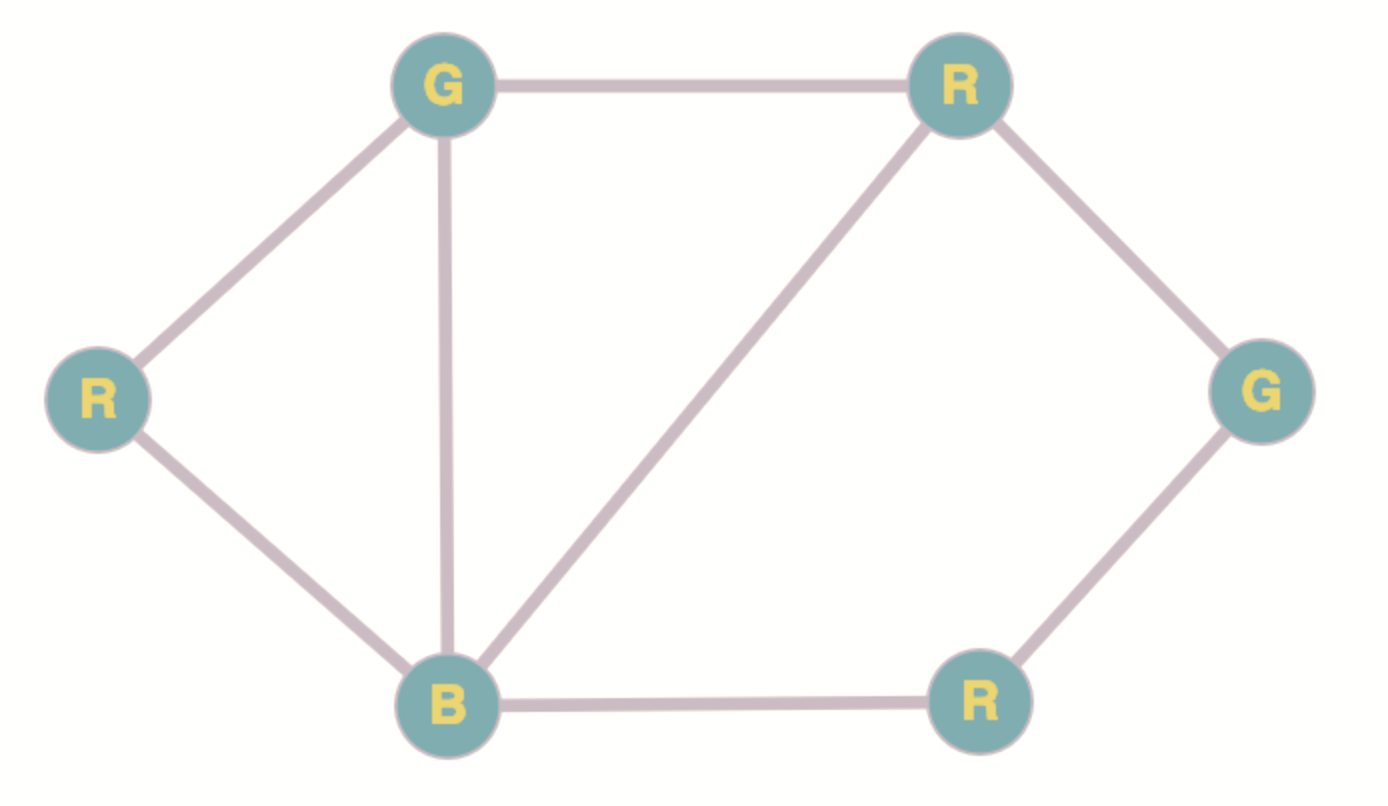
\includegraphics[width=0.4\linewidth]{3-1.png}
		\end{figure}
	
		\item 
		Since $v_1$, $v_2$ and $v_3$ are mutually connected and $v_1 = R$, $v_2$ and $v_3$ must be one $G$ and one $B$. Because $v_4$ is connected to $v_2$, $v_3$ and $v_6$, which are all three different colors, there is no color left for $v_4$. Thus, the graph cannot be coloring using three colors if $v_1 = v_5 = R$.
	\end{enumerate}

	\item [4.]
	Denote the hand shaking system as $G=(V, E)$ where $V$ represents the set of all people and $E$ represents the set of handshakes of two people. Then the degree of a vertex is the number of time a person shook hands. According to the degree sum formula, we have
	\[
	\sum_{v\in V} \deg(v) = 2\abs{E}
	\]
	Thus, the sum of individual handshakes is always twice the number of handshakes, which is always even.
	
	\item [5.]
	\begin{enumerate}
		\item 
		A minimum vertex cover can be $S=\{v_2, v_4, v_5\}$.
		
		\item 
		The problem can be modeled mathematically as an undirected graph $G=(V, E)$ where
		\begin{align*}
			V &= \{v_i\}, \quad i=1,2,\dots,5\\
			E &= \{(v_1, v_2), (v_2, v_3), (v_3, v_4), (v_3, v_5), (v_4, v_5)\}
		\end{align*}
		Let $x_i \in \{0,1\}, x=1,2,\dots,5$, s.t.
		\[
		x_i = 
		\begin{cases}
		0, & v_i \text{ is not chosen}\\
		1, & v_i \text{ is chosen}
		\end{cases}
		\]
		Then the problem is to
		\[
		\text{Min. } \sum_{i = 1}^{\abs{V}} x_i
		\]
		subject to
		\[
		x_i + x_j \ge 1, \forall (v_i, v_j) \in E
		\]
	\end{enumerate}
	
	\item [6.]
	The problem can be modeled mathematically as a directed graph $G=(V, E)$ where
	\begin{align*}
		V &= \{s, a, b, c, d, t\}\\
		E &= \{(s, a), (s, b), (a, b), (a, c), (b, c), (b, d), (c, d), (c, t), (d,t)\}
	\end{align*}
	The flow from $i$ to $j$ can be denoted as $x_{ij}, i,j\in V$. Then the problem is to
	\[
	\text{Max. } s = \sum_{(s, i)\in E} x_{si}
	\]
	Because the amount flow into and flow out of a vertex should be equal, nonnegative and within corresponding capacity ($c_{ij}, (i,j)\in E$), the objective function is subject to
	\begin{align*}
		\sum_{(i, j)\in E} x_{ij} =  \sum_{(j, k)\in E} x_{jk},& \quad \forall j\in V\backslash\{s, t\}\\
		0 \le x_{ij} \le c_{ij},& \quad \forall (i,j)\in E
	\end{align*}
	Solving it, we have $s=8$.
\end{enumerate}

\end{document}

